%GiG
\documentclass{beamer} 
\usetheme{Copenhagen}
\setbeamertemplate{navigation symbols}{}
\setbeamertemplate{headline}{}
\DeclareMathOperator*{\argmax}{arg\,max}

\usepackage{hyperref}
\definecolor{azure}{rgb}{0.0, 0.5, 1.0}
%\newcommand{\tblue}[1]{\textcolor{blue}{#1}}
\newcommand{\tblue}[1]{{\Large {\textcolor{azure}{#1}}}}
\newcommand{\hred}[1]{{\textcolor{red}{#1}}}

\title[Saravanan Thirumuruganathan] 
{Lecture 3: Lower Bounds for Sorting, Linear Time Sorting Algorithms}

\author[CSE 5311] 
{Instructor: Saravanan Thirumuruganathan}

\date[] 

\begin{document}

\begin{frame}
  \titlepage
\end{frame}

%\begin{frame}{Outline}
%  \tableofcontents
%  % You might wish to add the option [pausesections]
%\end{frame}

\section{Outline}

\begin{frame}
\frametitle {Outline}
\begin{enumerate}
\item Lower bound for Comparison based Sorting Algorithms
\begin{itemize}
    \item Concept of Lower Bounds
    \item Decision tree model of complexity
\end{itemize}
\item Linear Time Non-Comparison based Sorting Algorithms
\end{enumerate}
\end{frame}

\begin{frame}{In-Class Quizzes}
\begin{itemize}
\item {\Large {\bf URL:}} {\LARGE \bf \url{http://m.socrative.com/}} 
\item {\Large {\bf Room Name:} {\LARGE \bf 4f2bb99e}}
\end{itemize}
\end{frame}

\section{Lower Bounds for Sorting Algorithms}

\begin{frame}{Sorting Problem}
\begin{itemize}
\item {\bf Input:} A sequence of $n$ numbers $\langle a_1, a_2, \ldots, a_n \rangle$
\item {\bf Output:} A permutation (reordering) $\langle a_1', a_2', \ldots,  a_n' \rangle$ of the input sequence
such that $a_1' \leq a_2' \leq \ldots \leq a_n'$ 
\item {\bf Example:} $\langle 4, 2, 1, 3, 5\rangle$ to $\langle 1, 2, 3, 4, 5\rangle$    
\item Assume distinct values (doesn't affect correctness or analysis)
\end{itemize}
\end{frame}


\begin{frame}{Sorting Algorithms - So Far}
\begin{itemize}
\item We started with elementary algorithms (Bubble, Selection, Insertion) that were $O(n^2)$ in worst case
\item Using some clever ideas (such as D\&C), we have some algorithms (Merge and Quick) that are $O(n \lg n)$
\item Question: Can we do better? Or have we hit some fundamental computational limit?
\end{itemize}
\end{frame}



\begin{frame}{One Slide Summary}
\begin{itemize}
\item Comparison based sorting algorithms require $\Omega(n \lg n)$
\item In other words, for some input every comparison based sorting algorithms will require $\Omega(n \lg n)$
\item Result does not apply for non-comparison based algorithms which can be more efficient under some circumstances
\end{itemize}
\end{frame}



\begin{frame}{Lower Bound of an Algorithm\footnote{Slides from MCS/CS 401 slides by Roy M. Lowman}}
\begin{itemize}
\item Algorithm $A$ has a lower bound $\Omega(T(n))$ if there exists an input of size $n$ on which $A$ takes $\Omega(T(n))$ time
\item Lower bound is not the same as best case!
\item Insertion sort has lower bound $\Omega(n^2)$ (if the array is reverse sorted)
\item Merge sort has lower bound $\Omega(n \lg n)$ (for reverse sorted array and many other inputs)
\item Finding lower bound of an algorithm is relatively easy
\end{itemize}
\end{frame}



\begin{frame}{Lower Bound of a Problem}
\begin{itemize}
\item Problem $P$ has a lower bound $\Omega(T(n))$ if for {\bf every} algorithm $A$ that solves $P$, 
there exists an input of size $n$ on which $A$ takes $\Omega(T(n))$ time
\item In general, very hard - has to hold for {\em all} algorithms (even those humans have not invented yet)
\item Lower bounds known for very few problems!
\item Typical Strategy: Restrict computation model
\end{itemize}
\end{frame}



\begin{frame}{Lower Bound of a Problem}
\begin{itemize}
\item $O(f(n))$ - upper bound
\item $\Omega(g(n))$ - lower bound
\item If $f(n)$ is not $g(n)$, then there is an ``efficiency gap'' - Opportunity for improvement!
\item For example, $O(n^2)$ for insertion sort versus $\Omega(n \lg n)$ for sorting
\end{itemize}
\end{frame}


\begin{frame}{Lower Bounds for Sorting}

{\bf Theorem:} Any Algorithm that sorts by {\bf only comparing} elements must take $\Omega(n \lg n)$ time in the worst case.
\end{frame}

\begin{frame}{Sorting As Permutation}
\begin{itemize}
\item Sorting is equivalent to finding a permutation 
\item Find the {\bf inverse} permutation (among all permutations) that will undo the original permutation
\end{itemize}
\begin{center}
    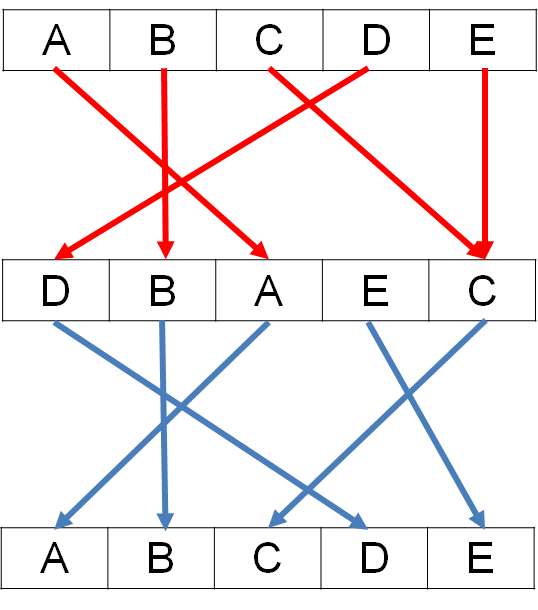
\includegraphics[scale=0.3]{sortingAsPermutation.png}
\end{center}
\end{frame}



\begin{frame}{Sorting As Permutation}
\begin{center}
    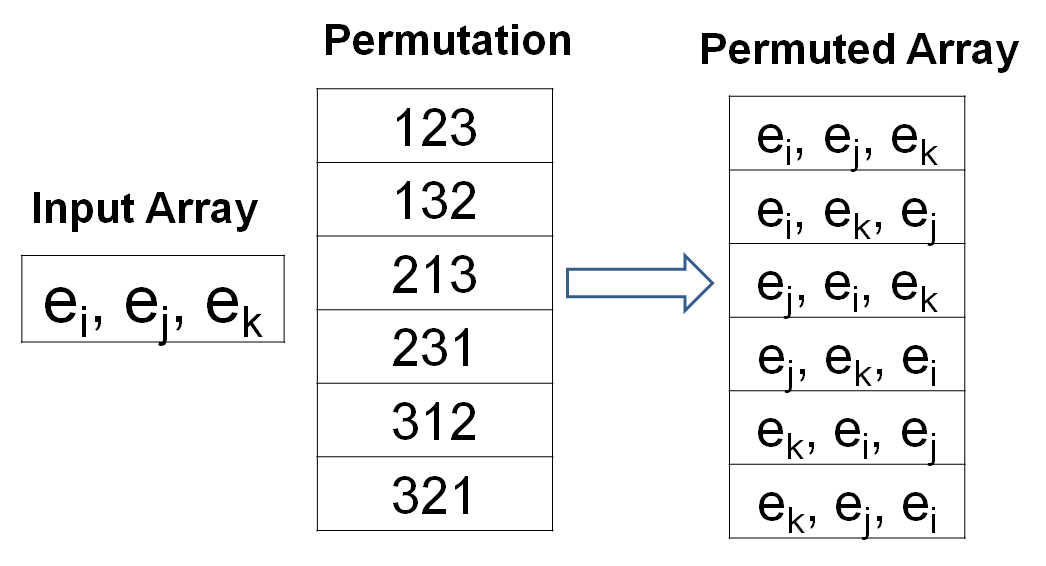
\includegraphics[scale=0.3]{sortingAsPermutation2.png}
\end{center}
\end{frame}


\begin{frame}{Quiz!}
\begin{itemize}
\item Suppose you an array $A$ with elements $\{1,2,3,4,5\}$. How many different arrays with distinct elements are possible?
\end{itemize}
\end{frame}



\begin{frame}{Quiz!}
Suppose you an array $A$ with elements $\{1,2,3,4,5\}$. How many different arrays with distinct elements are possible?
\begin{itemize}
\item You can choose any of $5$ elements for first position
\item You can choose any of $4$ elements (except the one chosen previously) for second position
\item And so on until you are left with no choice for last element
\item There are $5 \times 4 \times 3 \times 2 \times 1 = 5! = 120$ different arrays
\end{itemize}
\end{frame}



\begin{frame}{Decision Tree Model for Sorting\footnote{Figures from MCS/CS 401 slides by Roy M. Lowman}}
\begin{center}
    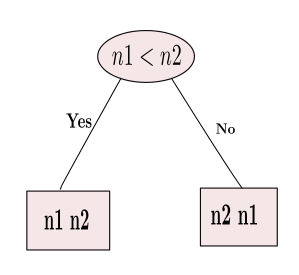
\includegraphics[scale=0.5]{sortingDTree2Elems.png}
\end{center}
\end{frame}

\begin{frame}{Decision Tree Model for Sorting\footnote{Figures from MCS/CS 401 slides by Roy M. Lowman}}
\begin{center}
    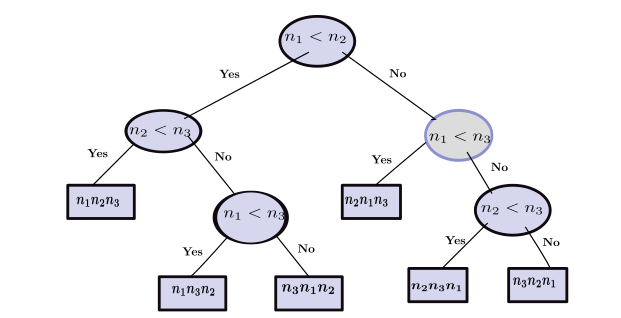
\includegraphics[scale=0.5]{sortingDTree3Elems.png}
\end{center}
\end{frame}


\begin{frame}{Decision Tree Model for Sorting\footnote{Figures from CLRS}}
\begin{center}
    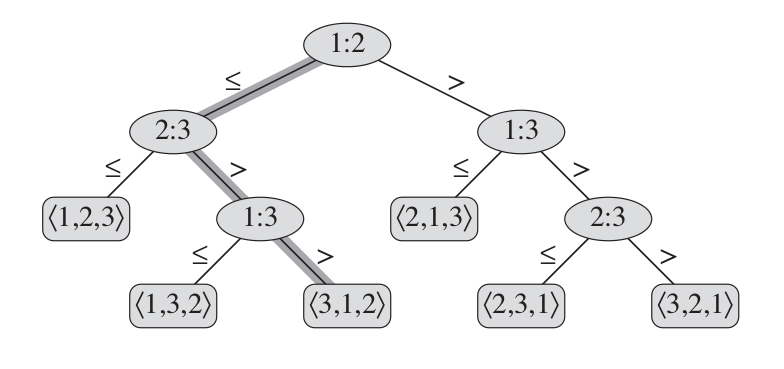
\includegraphics[scale=0.36]{sortingDTree3ElemsCLRS.png}
\end{center}
\end{frame}


\begin{frame}{Decision Tree Model for Sorting\footnote{Figures from CLRS}}
Sorting $\langle a_1 = 6, a_2 = 8, a_3 = 5 \rangle$ 
\begin{center}
    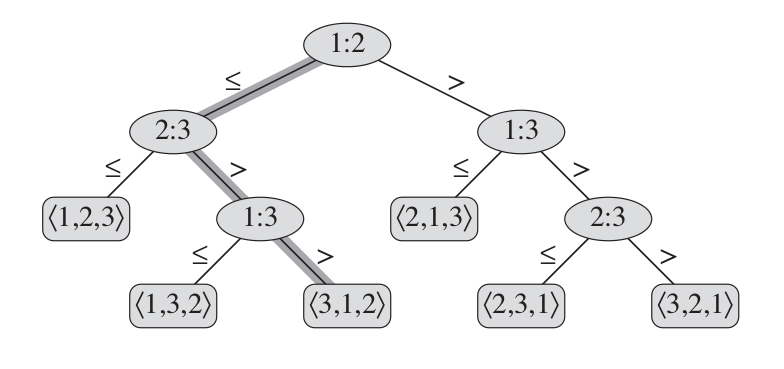
\includegraphics[scale=0.36]{sortingDTree3ElemsCLRS.png}
\end{center}
\end{frame}



\begin{frame}{Decision Tree Model for Sorting}
\begin{itemize}
\item {\em Every} comparison based sort algorithms can be modelled as a decision tree
\item Non-leaf (internal) nodes represent comparisons
\item Leaf nodes provide the permutation that will result in the sorted array
\end{itemize}
\end{frame}

\begin{frame}{Sorting Lower Bounds}
\begin{itemize}
\item Number of leaves in the decision tree must be at least $n!$ (why?)
\item Idea: Use $n!$ to get the lower bound
\item Height of a leaf node represents number of {\bf comparisons} made to sort a particular data represented by that node
\item Interpretation of Longest path length and Average path length?
\end{itemize}
\end{frame}


\begin{frame}{Sorting Lower Bounds}

{\bf Theorem:} Any Algorithm that sorts by {\bf only comparing} elements must take $\Omega(n \lg n)$ time in the worst case.

{\bf Proof:} 
\begin{itemize}
\item The tree has at least $n!$ leaves 
\item A binary with height $h$ has $\leq 2^h$ leaves
\end{itemize}

\begin{align*}
n!  &\leq 2^h \\
\lg n! & \leq \lg 2^h = h \lg 2 = h\\
~ & ~ \\
h   &\geq \lg (n!) \\
    &= \lg \prod_{i=1}^{n} i = \sum_{i=1}^{n} \lg i \\
    &= \Theta(n \lg n)\\
h   &= \Omega(n \lg n)
\end{align*}
\end{frame}



\begin{frame}{Sorting Lower Bounds}
\begin{itemize}
\item Any {\bf comparison } based sorting algorithms must take $\Omega(n \lg n)$ time in the worst case. 
\item Has major theoretical and practical implications
\end{itemize}
\end{frame}


\section{Linear Time Sorting Algorithms}

\begin{frame}{Linear Time Sorting Algorithms}
\begin{itemize}
\item Non-comparison based sorting algorithms
\item Side step the $\Omega(n \lg n)$ barrier
\item Counting, Radix and Bucket sort
\end{itemize}
\end{frame}


\begin{frame}{Counting Sort - Intuition}
\begin{itemize}
\item Suppose you are given a binary string (say $01110001$) and you want to sort it (to $00001111$).
\item Which algorithm would you use?
\begin{itemize}
    \item Bubble, Selection, Insertion sort
    \item Merge and Quick sort
\end{itemize}
\end{itemize}
\end{frame}


\begin{frame}{Counting Sort - Intuition}
\begin{itemize}
\item What about decimal numbers?
\item What about text with ASCII characters?
\item Handling complex objects and stability
\end{itemize}
\end{frame}


\begin{frame}{Counting Sort}
\begin{center}
    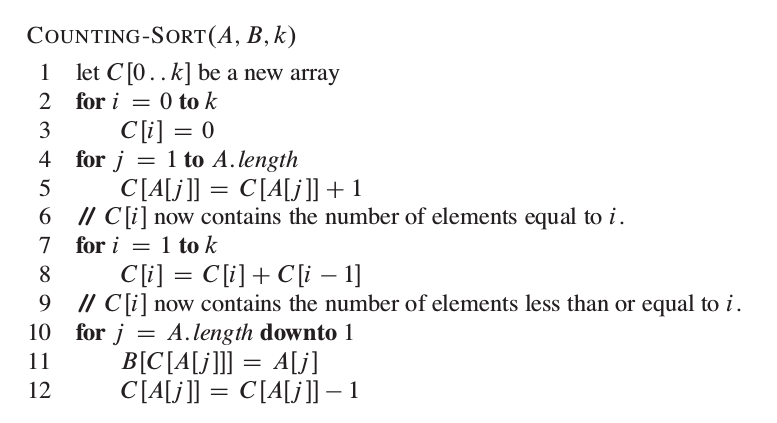
\includegraphics[scale=0.4]{countingSortPseudoCode.png}
\end{center}
\end{frame}


\begin{frame}{Counting Sort}
\begin{itemize}
\item For every key $j$, $1 \leq j \leq k$, store its frequency in $C[j]$
\item Then, change $C[j]$ to mean the number of keys $\leq j$
\item Use a clever trick to move items to the right place by traversing the array right to left
\item This trick is needed to ensure Stability - needed for Radix sort
\end{itemize}
\end{frame}



\begin{frame}{Counting Sort - Visualization}
\begin{itemize}
\item See URL \url{http://www.cs.miami.edu/~burt/learning/Csc517.101/workbook/countingsort.html} 
\end{itemize}
\end{frame}


\begin{frame}{Counting Sort - Analysis}
\begin{itemize}
\item Time Complexity : $O(n+k) = O(n)$ - Why?
\item Count sort is Stable - Why?
\item What prevents us from always using Counting sort?
\end{itemize}
\end{frame}


\begin{frame}{Count Sort - Results\footnote{\url{http://www.inf.ed.ac.uk/teaching/courses/ads/Lects/lecture8.pdf}}}
\begin{itemize}
\item Interesting Result 1:
\begin{itemize}
    \item Suppose you want to sort an array $A$ with $n$ elements. The keys are integers in the range of $1, \ldots, m$ where $m=O(n)$
    \item You can sort $A$ in $O(n)$ time
\end{itemize}
\item Interesting Result 2:
\begin{itemize}
    \item For any {\em constant} $k$, we can sort $n$ integers in the range $\{1, \ldots, n^k\}$ in $O(n)$ time
    \item Details soon!
\end{itemize}
\end{itemize}
\end{frame}


\begin{frame}{Radix Sort\footnote{\url{http://www.inf.ed.ac.uk/teaching/courses/ads/Lects/lecture8.pdf}}}
\begin{itemize}
\item Keys are sequences of {\em digits} in a fixed range $1, \ldots, k$, all of equal length $d$ 
\item Applications:
\begin{itemize}
    \item Sorting phone numbers by Area Code
    \item Sorting dates by Day, Month and Year (for e.g. Apache logs)
    \item Sort courses by course name and number
    \item Sorting social security number
\end{itemize}
\end{itemize}
\end{frame}

\begin{frame}{Radix Sort}
\begin{itemize}
    \item LSD Radix Sort
    \item MSD Radix Sort
\end{itemize}
\end{frame}

\begin{frame}[fragile]{LSD Radix Sort - PseudoCode}
\begin{verbatim}
Radix-Sort(A, d)
    for i = 1 to d
        use a stable sort to sort array A on digit i
\end{verbatim}
\end{frame}


\begin{frame}{LSD Radix Sort - Example\footnote{\url{http://www.cs.princeton.edu/~rs/AlgsDS07/18RadixSort.pdf}}}
\begin{center}
    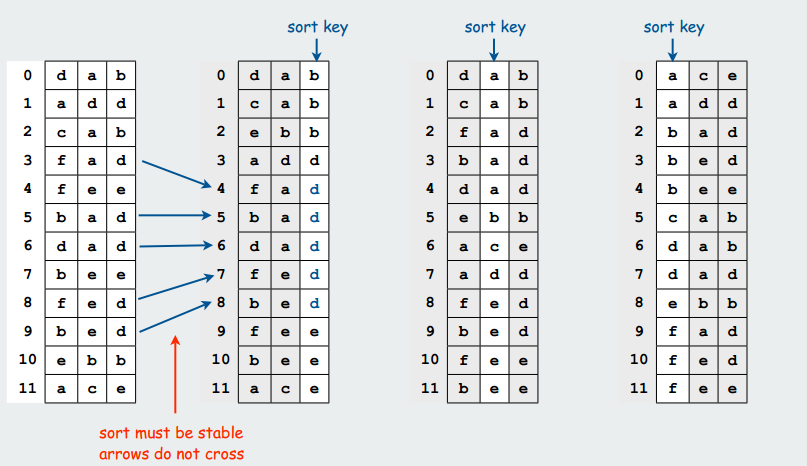
\includegraphics[scale=0.4]{radixSortEg1.png}
\end{center}
\end{frame}

\begin{frame}{Digression - Bucket Sort}
\begin{itemize}
\item See URL: \url{http://www.dcs.gla.ac.uk/~pat/52233/slides/RadixSort1x1.pdf} 
\end{itemize}
\end{frame}


\begin{frame}{LSD Radix Sort - Bucket Sort Perspective}
\begin{itemize}
   \item See URL: \url{http://www.cs.umanitoba.ca/~chrisib/teaching/comp2140/notes/003e_radixSort.pdf} 
\end{itemize}
\end{frame}

\begin{frame}{LSD Radix Sort - Why it works\footnote{\url{http://www.cs.princeton.edu/~rs/AlgsDS07/18RadixSort.pdf}}}
\begin{itemize}
\item Suppose you sorted the array based on LSD (digit $1$)
\begin{itemize}
    \item If two numbers {\bf differ} on first digit, Counting sort puts them in correct relative order
    \item If two numbers {\bf agree} on first digit, stability keeps in correct relative order
\end{itemize}
\item Consider the next step - sorting digit $2$ 
\begin{itemize}
    \item If two numbers {\bf differ} on second digit (or other digits), it doesn't matter what we do now
    \item If two numbers {\bf agree} on second digit (or other digits), stability ensures later passes wont cause any issues
\end{itemize}
\end{itemize}
\end{frame}


\begin{frame}{MSD Radix Sort\footnote{\url{http://www.cs.princeton.edu/~rs/AlgsDS07/18RadixSort.pdf}}}
\begin{itemize}
\item Partition array to $k$ pieces based on first digit
\item {\bf Recursively} sort array 
\end{itemize}
\begin{center}
    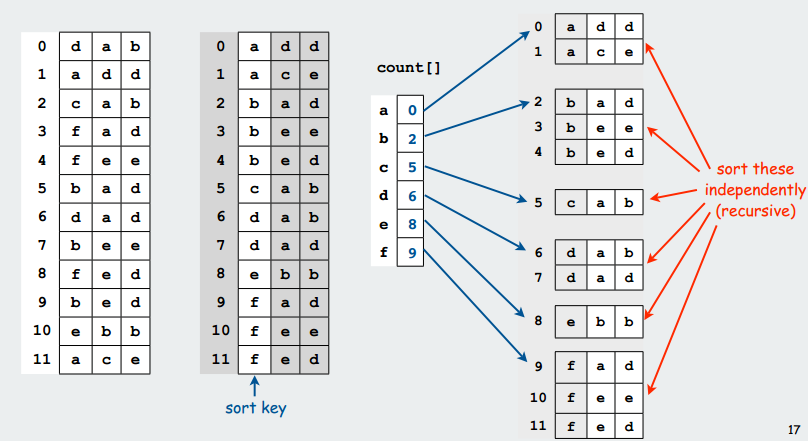
\includegraphics[scale=0.35]{msdRadixSortEg.png}
\end{center}
\end{frame}


\begin{frame}{LSD Radix Sort - Analysis}
\begin{itemize}
\item Given $n$ $d$-digit numbers in which each digit can take up to $k$ possible values
\item Radix-Sort correctly sorts them in $O( d(n+k) )$ time
\item {\bf if} the stable sort takes $O(n+k)$ time.
\end{itemize}
\end{frame}


\begin{frame}{Summary}

\tblue{Major Concepts:}
\begin{itemize}
\item Concept of Lower bounds
\item Lower bounds for Comparison based Sorting Algorithms
\item Decision tree model for Complexity Analysis
\item Linear Time Sorting Algorithms
\end{itemize}
\end{frame}


\end{document}

